% ============================================================================
% Capítulo 8 — Infraestrutura em nuvem e DevOps
% ============================================================================
\section{INFRAESTRUTURA EM NUVEM E DEVOPS}

\subsection{Execução local com contêineres}

A solução é executada localmente com dois contêineres: o banco SQL Server 2022 e
a aplicação Web/API. O \texttt{Dockerfile} utiliza construção em múltiplos
estágios -- imagem de SDK para compilar e publicar, imagem de runtime para
executar --, reduzindo o tamanho final e a superfície de ataque. O
\texttt{docker-compose.yml} declara a dependência entre os serviços, o
verificador de saúde do banco e as variáveis de ambiente necessárias.

O serviço da aplicação aguarda o banco estar saudável antes de iniciar e, no
ambiente de demonstração, aplica as migrations e o seed automaticamente. Para o
banco, o script \texttt{db/script-completo.sql} oferece uma alternativa
reprodutível em ambientes sem .NET. Essas duas formas de provisionamento foram
validadas: o script em banco limpo e as migrations em banco vazio.

\subsection{Integração e entrega contínuas}

O pipeline definido em \texttt{.github/workflows/ci.yml} é acionado em cada
envio para a linha principal, em branches de funcionalidade e em solicitações de
integração. As etapas são: restauração de dependências, compilação em modo
Release, execução dos testes com publicação dos resultados e construção da
imagem da aplicação. A escolha por falhar cedo -- compilar e testar antes de
publicar -- evita que artefatos quebrados cheguem ao ambiente de demonstração.

O fluxo adotado no desenvolvimento seguiu a mesma lógica em escala local: cada
incremento termina com compilação sem avisos, testes aprovados e commit em
português. Ao final, a árvore integrada apresentou 159 testes aprovados, sem
falhas, tanto no backend quanto no aplicativo mobile.

\subsection{Arquitetura de implantação em nuvem}

O plano de implantação utiliza serviços gerenciados do Microsoft Azure,
representados na Figura~\ref{fig:azure}. A aplicação é publicada no Azure App
Service para Linux (.NET 10) ou no Azure Container Apps; o banco migra para o
Azure SQL Database; as evidências fotográficas passam ao Blob Storage; e os
segredos são mantidos no Key Vault, referenciados por identidade gerenciada.

\begin{figure}[H]
  \centering
  \caption{Arquitetura de implantação em nuvem}
  \label{fig:azure}
  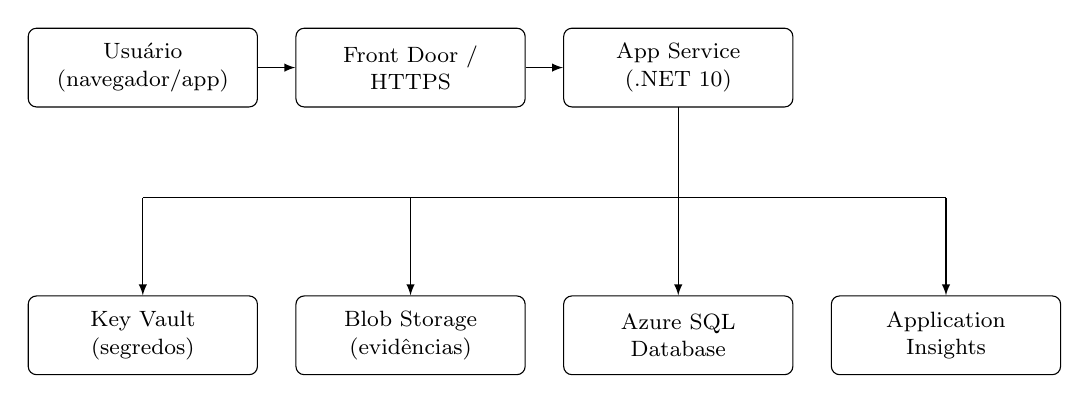
\begin{tikzpicture}[
    no/.style={draw, rounded corners=3pt, align=center, font=\fontsize{8.5}{10}\selectfont,
      minimum height=10mm, text width=27mm, inner sep=3pt},
    seta/.style={-latex, thin}
  ]
    \node[no] (user) at (0,9.0) {Usuário\\ (navegador/app)};
    \node[no] (fd)    at (3.4,9.0) {Front Door /\\ HTTPS};
    \node[no] (app)   at (6.8,9.0) {App Service\\ (.NET 10)};

    \node[no] (kv)    at (0.0,5.6) {Key Vault\\ (segredos)};
    \node[no] (blob)  at (3.4,5.6) {Blob Storage\\ (evidências)};
    \node[no] (sql)   at (6.8,5.6) {Azure SQL\\ Database};
    \node[no] (obs)   at (10.2,5.6) {Application\\ Insights};

    \draw[seta] (user) -- (fd);
    \draw[seta] (fd) -- (app);

    % Barramento de serviços consumidos pela aplicação.
    \draw (6.8,8.5) -- (6.8,7.35);
    \draw (0,7.35) -- (10.2,7.35);
    \draw[seta] (0,7.35) -- (kv.north);
    \draw[seta] (3.4,7.35) -- (blob.north);
    \draw[seta] (6.8,7.35) -- (sql.north);
    \draw[seta] (10.2,7.35) -- (obs.north);
  \end{tikzpicture}
  \fonte{elaborado pelo autor (2026)}
\end{figure}

\subsection{Monitoramento, escalabilidade e segurança}

A observabilidade combina logs estruturados, métricas de requisição e
identificador de correlação (\texttt{traceId}) devolvido nas respostas de erro.
Com Application Insights, é possível acompanhar latência, taxa de erro 5xx e
dependências, além de configurar alertas de disponibilidade.

A escalabilidade é horizontal (mais instâncias do App Service ou réplicas no
Container Apps) e vertical (ajuste de camada do Azure SQL). Como a aplicação é
sem estado -- cookie na Web e token na API --, não há necessidade de afinidade
de sessão; o armazenamento de evidências fora do disco local, já previsto,
completa esse desenho.

Na segurança, destacam-se: HTTPS obrigatório com HSTS em produção, Swagger
desabilitado fora do desenvolvimento, segredos fora do repositório, firewall do
banco restrito ao serviço de aplicação e backup automático do Azure SQL. O
checklist de produção reúne esses itens e deve ser verificado antes de cada
implantação.
